
\chapter{The alternation between full and elliptical answers}\label{sec:4}

\section{The ``immediacy” hypothesis} 

The corpus study conducted in \chapref{sec:3} revealed that subject focus can be expressed through both full and elliptical strategies in Spanish and French. Interestingly, while French clefts and Spanish postverbal subjects are the most common answer types, the second preferred option in both languages is an elliptical form — reduced clefts for French and fragments for Spanish — indicating that these structures are far from rare in spontaneous dialogues. 

As already discussed in \chapref{sec:2}, little has been said about why speakers prefer to use elliptical or full answers within the same conversation. 
Although several authors have pointed out that elliptical answers are often the most natural answer types in Q-A pairs with fast turns (e.g., \cite{belletti2005answering, belletti2008answering, lahousse2012word, vidal2019nota}), previous literature on this topic has been primarily concerned with the syntactic nature of these  structures, rather than with understanding why they appear and what determines the alternation with their full counterparts (however, see the recent doctoral thesis by \cite{bourgoin2022corpus}). 
\textcite{belletti2008cp}, for instance, analyzes reduced clefts as cleft sentences whose relative clause is not uttered for discourse-related reasons. In particular, she argues that reduced clefts are the most felicitous focus-marking strategy for the subject in French when the question \textbf{immediately} precedes the answer, as in (\ref{ex:4:1}), already illustrated in \chapref{sec:2}, that I report here:

\begin{exe}
	\ex \label{ex:4:1}
	\begin{xlist}
		\ex \textit{Qui} (\textit{est-ce que qui}) \textit{a parlé?}\\
		`Who spoke?'
		\ex \textit{C'est} {[\textit{Jean}]\textsubscript{\textsc{foc}}} \normalsize(\textit{qui a parlé}).\\
		`It is Jean (who spoke).' \hfill \parencite[192]{belletti2008cp}   
	\end{xlist}
\end{exe} 


Although a full cleft would not be ungrammatical, its use in the same context would probably be judged as infelicitous by many speakers, since uttering the relative clause would lead to a redundant repetition of the proposition already contained in the immediately-preceding question. Along the same lines, \textcite{katz2000categories} argues that such abbreviated responses are possible when the relative clause is highly activated due to having just been mentioned (e.g., in the case of an immediately-preceding question or assertion). 

These claims suggest that the syntactic form used to express focused subjects in dialogues may be influenced by the type of QUD (explicit or implicit) that triggers them. If a reduced cleft is an appropriate response when the question immediately precedes the answer, it naturally leads to the question of how responses are structured when the question does not directly precede the answer or is implicit, as is often the case in spontaneous speech. In other words, if immediately preceding questions tend to elicit elliptical answers, one would expect an association between non-immediately-preceding or implicit questions and full answers.
If this is the case, the factors determining the alternation between full and elliptical answers may be tied to the degree of activation of the background proposition, as suggested by \textcite{katz2000categories}. However, this assumption has not yet been empirically tested. 

 In the literature on information structure, the concept of activation is often associated with referential entities and referential choice. It is well known, for instance, that the level of activation of the referents in discourse determines the morphological form through which these referents are expressed, and that there is an inverse relationship between the level of activation of a referent and the form with which  such a referent appears.  In other words, the more recently an entity has been mentioned, the more accessible it still is in the discourse model, and the higher the likelihood that the speaker will use a pronominal or zero form \parencite{givon1983topic}. Givón’s (\citeyear{givon1983topic}) seminal work on topic continuity has pointed out that ``the cross-linguistic generalization is that less “coding material” (or less phonetic bulk) corresponds to more accessible referents, while more coding material corresponds to less accessible referents” \parencite[18]{givon1983topic}. 
Such an inverse relationship has been theorized in the Accessibility Theory \parencite{ariel1988referring} as well, according to which the more \say{informative, rigid and unattenuated an expression is, the lower the degree of accessibility it codes, and vice-versa, the less informative and rigid and the more attenuated the form is, the higher the accessibility it codes} \parencite[32]{ariel2001accessibility}. The term ``informativity” refers in this case to the amount of lexical information. Thus, highly accessible referents would be more likely expressed by pronouns, while less accessible referents would be associated to full lexical NPs. \textcite{ariel2001accessibility} identifies a hierarchy of accessibility that can be represented as the following referring expressions scale:

\ea \label{ex:4:2}
 {\large  ø\footnote{Zero anaphora in pro-drop languages.} $>$  Overt \ pronoun $>$  Full \ NP $>$  ... $>$ }
  \z

The more a referent is activated in the discourse, the more its referring form will be minimal or short, like the case of zero anaphora (ø) in pro-drop languages, or of overt pronoun in non-pro drop languages. Conversely, the less activated a referent is in discourse, the higher will be the likelihood for this referent to be expressed by forms which are found on the right part of Ariel's (\citeyear{ariel2001accessibility}) scale.

The Common Ground (henceforth CG) includes both referents and propositions. Speaker and hearer continually share and update a communicative space that contains these entities and the propositions associated with them. Therefore, if there is an inverse relationship between the activation of referents and the amount of morphological material used to express them, propositions might follow the same pattern. Since propositions, like referents, can vary in their level of activation within the discourse, it is reasonable to hypothesize a similar activation scale for propositions, based on the principle discussed above: 

\ea \label{ex:4:3}
  {\large Deletion $>$ Full\ realization}
  \z

Thus, a highly activated proposition is more likely to be omitted (in cases of deletion), while a less activated proposition is more likely to be fully realized. It is important to note that no strict one-to-one correlation is expected between the degree of activation and the expression or omission of a proposition. Instead, these relationships are predicted to be probabilistic, representing tendencies rather than categorical grammatical rules.
In a dialogical setting, the presupposition is generally contained in the preceding QUD. 

According to \textcite{lambrecht1996information}, the use of an information question is appropriate only if the open proposition resulting from removal of the question expression (the wh-element) from the sentence is pragmatically presupposed in the discourse. In other words, a question like `Who ate the cookie?' evokes the assumption that the addressee can identify the particular cookie the speaker has in mind, and accepts the fact that some individual ate this cookie as uncontroversial  (except in the case of a rhetorical  question, suggesting the answer `No one').
This implies that in case of immediately-preceding questions, where the answer directly follows the question, the proposition is highly activated. Conversely, with questions that do not precede the answer or are implicit, the level of activation of the proposition decreases. Following this line of argumentation, I formulated the following hypothesis:

\ea
\textbf{H1}: Speakers tend to use elliptical answers when the preceding QUD is immediate, while full answers are preferred when the QUD is either implicit or not immediate.\\
\z

The reader may have noticed that I postulate three possible levels of activation of the Background material (immediate, distant, implicit) and only two possible outcomes (deletion vs. full realization). While a more detailed analysis that identifies an intermediate level (e.g., pronominalization) would have been ideal, a pilot study conducted on the same corpus revealed that a third level could not observed. In principle, a realized but distant QUD should have a higher degree of activation than an unrealized (implicit) QUD. However, the pilot study revealed that this distinction does not affect the types of answers these questions elicit, as both implicit and distant QUDs resulted in the same outcomes. The decision to exclude a third level in my dependent variable is thus empirically motivated.

In order to test H1, a second corpus analysis was carried out, using the data that resulted from the corpus query reported in \chapref{sec:3}. The results of this study demonstrate that the level of immediacy of the preceding QUD and, hence, the degree of activation of the background proposition indeed has an effect on the alternation between full and elliptical answers. It also shows, however, that such an effect is different for the two languages: while French speakers tend to avoid using full forms in the case of immediately-preceding QUDs, Spanish speakers are less sensitive to this tendency. Conversely, in the case of distant or implicit QUDs, both French and Spanish speakers exhibit a clear preference for expressing more material, i.e., to employ fuller forms. I present an account of these findings in terms of economy of the language, showing that the choice of the sentential form is, to some extent, ruled by principles such as ``The Principle of Least Effort” \parencite{zipf1949human} and ``The Principle of Communicative Efficiency” \parencite{LevshinaMoran+2021, Levshina_2022}.

Although the results of this study are not surprising, the chapter presents several innovative points: i) it tests claims that have so far been made only at a theoretical level, ii) it stresses the importance of the activation of propositions in the CG and how this has an impact on speakers' linguistic expression, and iii) it provides a new method of operationalizing the activation of the QUD, by identifying three levels of distance (immediate, non-immediate, implicit).
The details of the corpus analysis are illustrated in the following sections: \sectref{sub:5.2} reports on the methodology of the study; \sectref{sub:5.3} and \sectref{sub:5.4} show the results of the analysis. Finally, \sectref{sub:5.5} discusses the findings from a comparative perspective. 


\section{Methodology} \label{sub:5.2}
In this section, I report the design of the study and the criteria for the annotation of the items. The goal is to investigate whether the realization or the deletion of the background proposition contained in the answer (dependent variable) is influenced by the immediacy of the preceding QUD (independent variable). The material consists of the answer types extracted  from the previous corpus query (\chapref{sec:3}) and their corresponding QUD. As illustrated in \chapref{sec:3}, Spanish speakers produced a total of 352 subject foci, and French speakers 436. 
Both the answer types and the QUDs were annotated according to the criteria listed in the following sections.

\subsection{Annotation of answer types} \label{sub:5.2.1}
\largerpage
The corpus study reported in the previous chapter has demonstrated that each language possesses five different strategies to express narrow focus on the subject. Although syntactically different, these structures can be grouped into two categories: i) answers with a focused subject and an overt background proposition; and ii) answers where only the focused subject is uttered. To the first category belong postverbal subjects, in situ foci and cleft constructions for the Spanish dataset, while the French data consists of clefts, in situ foci, and, although very scarce, dislocations.
The second category, on the other hand, includes fragments and reduced clefts for both languages. The tables below report the counts for each category and each language.

\begin{table}
\caption{Spanish}
\begin{tabularx}{0.8\textwidth}{Q >{\arraybackslash}X}
\lsptoprule
\textbf{Full answers} & \textbf{Elliptical answers} \\
\midrule
Postverbal subjects (N=167) & Fragments (N=102) \\
In situ (N=33) & Reduced clefts (N=21) \\
Clefts (N=29) & \\
\midrule
\textbf{Total} = \textbf{229} & \textbf{Total} = \textbf{123} \\
\lspbottomrule
\end{tabularx}
\end{table}

\begin{table}
\caption{French}
\begin{tabularx}{0.8\textwidth}{Q >{\arraybackslash}X}
\lsptoprule
\textbf{Full answers} & \textbf{Elliptical answers} \\
\midrule
Clefts (N=220) & Reduced clefts (N=137) \\
In situ (N=41) & Fragments (N=31) \\
Dislocations (N=7) & \\
\midrule
\textbf{Total} = \textbf{268} & \textbf{Total} = \textbf{168} \\
\lspbottomrule
\end{tabularx}
\end{table}



 The category of full answers received the tag \textsc{complete}, while elliptical answers were coded as \textsc{elliptical}.

\subsection{Annotation of QUDs} \label{sub:5.2.2}

Each answer type had already been extracted together with the implicit or explicit corresponding QUD. In this step, I annotated the QUDs, distinguishing three levels of annotation for the QUD type:

\subsubsection{Immediate QUD}
The case of the immediate QUD is a prototypical Q-A pair with a fast turn. The question is explicitly uttered, it directly precedes the answer, and is thus easily retrievable. This type of question has been annotated as \textsc{immediate}. Examples are provided in (\ref{ex:4:5}) and (\ref{ex:4:6}) for French and Spanish, respectively. Both in the QUD and in the answer, the BG proposition is underlined for better visibility:

 \ea\label{ex:4:5} French
\ea \textit{En fait,} \uline{\textit{il y avait}} \textit{qui} \uline{\textit{dans l'immeuble}} \textit{quand ça s'est passé?}\\
 ‘So, who was in the building when all this happened?'
\ex \textit{Alors en fait il y avait} {[\textit{la grand-mère du dessus}]\textsubscript{\textsc{foc}}} \normalsize \uline{\textit{qui était là}}.\\
‘So, actually, there was the old lady from upstairs who was there.' 

\hfill (\textit{sgs} French, 9/261-262)   
\z \z

\ea \label{ex:4:6} Spanish
\ea 	\textit{¿Quién} \uline{\textit{vive por ahí}}?\\
 ‘Who lives there?'
\ex  \uline{\textit{Vive}} {[\textit{un señor importante}]\textsubscript{\textsc{foc.}}} \normalsize\\
‘An important man lives there.' \hfill (\textit{sgs} Spanish, 3/18-19)    
\z \z

\subsubsection{Distant QUD}
The second type is less straightforward. The question that triggers the focused subject does not immediately precede it. Typically, there are intervening utterances between the QUD and its answer. The basic idea here is that multiple utterances in the discourse model compete for the limited resource of activation. The criterion of intervening utterances as a measure of decreased accessibility (or activation decay) of the proposition is also parallel to a factor that has been claimed to affect referential choice, namely the distance between the anaphora and its antecedent measured by the number of intervening, competing referents (e.g., \cite{arnold2007effect}).
In the case of referents, competition would make the speaker express more coding material to refer to that particular entity. Building on these claims, I assume that the presence of competing utterances would contribute to the activation decay of the BG proposition. This type is coded as \textsc{distant}. Consider (\ref{ex:4:7}) and (\ref{ex:4:8}):

\ea \label{ex:4:7} French
\ea \textit{Et les enfants, qui }\uline{\textit{s’en occupe}}?\\
`And who takes care of the children?'
\ex \textit{Donc, en ce moment, ils sont pas là.}\\
`So, at the moment, they are not there.'
\exi{b.} \textit{Ils sont en vacances.}\\
`They are on holidays.'
\exi{b.} \textit{Sinon, c'est} {[\textit{une nourrice}]\textsubscript{\textsc{foc}}} \normalsize \uline{\textit{qui les garde le soir}}.\\
‘Usually it's a babysitter that takes care of them at night.' 

\hfill (\textit{sgs} French, 14/133-136)    
\z \z 

\ea \label{ex:4:8} Spanish
\ea \textit{¿Qué gente} \uline{\textit{entra en esa casa, además de la familia}}?\\
`Which other people have accessed to that house apart from his family?'
\ex \textit{Pues sí que tienen mujer de la limpieza.}\\
`Well, he has a cleaning lady.'
\exi{a.} \textit{¿Quién tiene llaves?}\\
`Who has the key?'
\exi{b.} \textit{m}.\\  
`m.'
\exi{b.} \textit{Tienen la mujer de la limpieza.}\\ 
`They have the cleaning lady.'
\exi{b.} \textit{Después, estos días también} \uline{\textit{han venido}} {[\textit{el electricista, el lampista}]\textsubscript{\textsc{foc.}}}\normalsize\\
‘Then, these days, the electrician, the plumber came as well.' 

\hfill (\textit{sgs} Spanish, 40/127-132)   
\z \z 

 In (\ref{ex:4:7}), it is possible to see that the QUD \textit{Qui s'en occupe?} `Who takes care of the children?' does not immediately precede the answer. Before answering the actual QUD, speaker B utters additional information, which represents not-at-issue content, and intervenes between the question and the answer, thus decreasing the level of activation of the background proposition contained in the question (i.e., to take care of the children). Similarly, in the Spanish example in (\ref{ex:4:8}), speaker A asks who had access to the apartment, apart from the family. Speaker B answers that the family has a cleaning lady. The speaker specifies that the cleaning lady can enter the apartment, but does not clearly say if she had access to the flat during those days. Rather, the actual answer to the original question is provided at the end of the dialogue (i.e., the electrician, the plumber).

 \subsubsection{Implicit QUD}
 \largerpage[2]
 The third type of QUD is more complicated. It is not uncommon in spontaneous speech to find implicit material. Rather, many questions in dialogues are not uttered explicitly. Sometimes, speakers anticipate possible questions of their interlocutors, and this results in more spontaneity in the conversation. When the QUD is implicit, it has to be retrieved by looking at the preceding utterances and at the answer itself.
Reconstructing an implicit QUD, however, can potentially be an arbitrary process, especially when it comes to marked constructions such as clefts, which usually trigger specific IS-interpretations (e.g., focus-background). To avoid circularity and manage a correct retrieval of the QUD, I followed the criteria listed in the QUD guidelines by \textcite{riester2018annotation, riester2019constructing}.

The authors propose a series of constraints that regulate the reconstruction of the QUD, and allow its derivation from the preceding discourse context. The constraints are derived from the focus literature of the past decades, in particular, \textcite{rooth1992theory}, \textcite{schwarzschild1999givenness} and \textcite{buring2009towards}. For instance, implicit QUDs must be answerable by an assertion that they immediately dominate (Q-A-Congruence constraint), they must contain as much given material as possible (Maximize-Q-Anaphoricity constraint) and can only consist of given or at least highly salient information (Q-Givenness constraint). Consider the example in (\ref{ex:4:9}) taken from \textcite{riester2019constructing}:

\ea \label{ex:4:9}
\ea And all I can say is that his condition was extremely bad during his last year.\\

\ex He literally suffocated. \hfill \parencite[9]{riester2019constructing}     
\z \z

 The assertion in (\ref{ex:4:9}b) gives rise to a set of alternative QUDs, such as:
\begin{itemize}
	\item Q1: What happened?
	\item Q2: What about him?
	\item Q3: Who literally suffocated?
	\item Q4: Who owns a bicycle?
\end{itemize}


According to the Q-A-Congruence constraint, Q4 is ruled out because it cannot be answered by the assertion that it immediately dominates. Q1 is also excluded because of the Maximize-Q-Anaphoricity constraint, which states that the QUD must contain as much given or salient material as possible, and a question like Q1 does not contain any of the given material found in the assertion. Finally, the Q-Givenness constraint, according to which an implicit QUD cannot introduce new material (except from function words and wh-particles), excludes Q3, because the fact of being ‘literally suffocated’ is new information, and fails to provide a link with the previous context. Conversely, the personal pronoun ‘he’ is connected to the previous sentence by virtue of reference continuity (the possessor 
`his' in ‘his condition' in (\ref{ex:4:9}a)). Q2 is hence the optimal candidate as the implicit QUD of the assertion contained in (\ref{ex:4:9}b).

\textcite{riester2018annotation} and \textcite{riester2019constructing} also note that, usually, there is no single way of formulating implicit QUDs, since languages allows for synonymous formulations. In other words, the assertion contained in (\ref{ex:4:9}b) could as well be an answer to a question such as ‘how bad was his condition/situation?’. Nevertheless, these constraints provide specific criteria for the retrieval of the implicit question. This type of QUD is tagged as \textsc{implicit}. Examples are provided in (\ref{ex:4:10}) and (\ref{ex:4:11}):

\ea \label{ex:4:10} French
\ea \textit{Mais il y avait} \uline{\textit{une soirée}}.\\
`But there was a party.'
\ex \textit{mh}.\\
`m.'
\exi{a.} \textit{Donc, justement, c'est} {[\textit{les voisins du haut}]\textsubscript{\textsc{foc}}} \normalsize \uline{\textit{qui ont organisé cette soirée}}.\\
`So, it was precisely the upstairs neighbors that organized this party.' \hfill (\textit{sgs} French, 59/ 338-340)    
\z \z 
\hfill (\textbf{Implicit QUD}: Who organized the party?)

\ea \label{ex:4:11} Spanish
\ea \textit{Económicamente le iba bien y así?}\\  
`Was s/he doing financially well and so?'
\ex \textit{Sí, a ver,} \uline{\textit{estos pisos}} \textit{son un poco caros.}\\
`Yes, well, the apartments here are somewhat expensive.'
\exi{b.} \textit{Y,} \uline{\textit{vivían}} \textit{sólo} {[\textit{dos personas}]\textsubscript{\textsc{foc.}}}\normalsize\\
`And only two people lived (in this apartment).' 

\hfill (\textit{sgs} Spanish, 15/183-185)
\z \z
\hfill (\textbf{Implicit QUD}: How many people lived in this apartment?)\medskip


Let us try to reconstruct the implicit QUD answered by the assertion \textit{C'est les voisins du haut qui ont organisé cette soirée} `It is the upstairs neighbors who organized this party' contained in (\ref{ex:4:10}), considering both the material in the assertion and the context preceding it. To avoid being biased by morphosyntactic cues, I do not take into account  the fact that the assertion is a cleft sentence, and I only build on the semantic content of the dialogue.
The Q-A-Congruence constraint rules out an implicit QUD such as ‘What about him?’ because it would not be semantically congruent with the answer. 

The referent \textit{les voisins du haut} `the upstairs neighbors' is discourse-new, and, therefore, cannot be part of the background proposition.\footnote{Recall that, according to the Q-Givenness constraint, implicit QUDs cannot contain new material and must consist of given or highly-salient material.} In other words, a QUD such as ‘What about the upstairs neighbors?’ is excluded as well. The referent \textit{soirée} `party', however, has already been mentioned in the preceding utterance. Its co-reference with its antecedent is also attested in the use of the demonstrative \textit{cette} `this'. 
Applying the Q-Anaphoricity constraint, I assume that the implicit QUD must somehow contain this referent. 
The verb \textit{organiser} `to organise' has not been previously mentioned either. However, the word \textit{soirée} `party' activates a series of possible QUDs in the mind of the hearer, such as `Who came to the party?', `How many people?', `How was the music?', `How was the food?' or `Who organized this party?'.

Among the different possibilities, it seems plausible that the last question (Who organized this party?) is the most felicitous in context. Speaker A wants to know about possible noises in the building, speaker B informs speaker A of a party, and assumes that speaker A wants to know who are the people responsible for the party/noise of that particular evening. 

Thus, it is possible to assume that \textit{organiser} `to organize', although not properly given, is highly salient, and that its salience is activated by the referent \textit{soirée} `party'. For this reason, it can be considered part of the implicit QUD. The discourse marker \textit{justement} `precisely' is additional evidence of the link between the current assertion and the previous context, proving that ‘Who organized the party?’ is a sub-question of the main QUD \textit{Est-ce qu'il y a eu des problèmes de bruit?} `Had there been
problems with respect to noise?'. Speaker A is thus signalling that s/he is providing additional information with respect to the noise heard that evening.
In summary, the implicit QUD can contain material, such as \textit{soirée} and \textit{organiser}, but cannot include brand-new information, such as the upstairs neighbors, which in turn can be considered the focus of the sentence, i.e., the part of the assertion that satisfies the wh-variable in the implicit QUD.
Therefore, I assume that the cleft sentence in (\ref{ex:4:10}) has a classical focus-background partition, with the clefted element being the focus and the relative clause the background proposition.

Similarly, in the Spanish example (\ref{ex:4:11}), speaker A is asking about the economic situation of the neighbor in question. Speaker B provides evidence of their wealth by informing speaker A that the apartments in the building are very expensive and that there were only two people living in that particular flat (and hence only two people paying rent). As was the case in the French example with the concept of `party', the word \textit{piso} `apartment' is salient because it evokes a series of possible QUDs. These might include, for instance, `Who lived in the apartment?', `For how long?' or `How many people lived there?'. Speaker A already knows that a couple lives in the apartment in question. What he/she does not know, however, is if they share rent with someone else. Speaker A, thus, informs him/her that only two people live in that flat.

The three types of QUDs are illustrated in \tabref{tab:5.3} together with their corresponding tags.

\begin{table}
    
   \begin{tabularx}{\textwidth} {
   Q
   Q
     Q  }
 \lsptoprule
 \textbf{Immediate QUD} & \textbf{Distant QUD} & \textbf{Implicit QUD} \\
\midrule
\small The question immediately precedes the answer.  & \small The question does not immediately precede the answer. &  \small The question is implicit.  \\
\midrule
Tag: \small \textsc{immediate} & Tag: \small \textsc{distant} & Tag: \small \textsc{implicit} \\
\lspbottomrule
\end{tabularx}\\
    \caption{QUD types}
    \label{tab:5.3}
\end{table}

\subsubsection{Modality of the QUD}%\todo{added subsubsection title}

Both in the French and in the Spanish dialogues, it has been observed that the types of explicit QUDs could be of two modalities: wh-question and yes-no questions. These two question types are intrinsically different not only with respect to their syntactic configuration, but also with regard to the pragmatic inference they trigger. While wh-questions contain an overt wh-element which, according to the Alternative Semantic Framework \parencite{rooth1985association, rooth1992theory}, must be filled with one (or more) possible alternatives (i.e., the focus), in yes-no questions (also called polarity questions), the variable is, in principle, satisfied by the polarity item `yes' or `no'. 
Typical of spontaneous speech, however, is the phenomenon of over-answering yes-no questions, i.e., of generating extended responses that provide additional information to yes-no questions that pragmatically must be interpreted as wh-questions \parencite{wahlster1983over, steensig2013yes}. Indeed, a cooperative speaker has the ability to recognize when it is appropriate to provide more than a mere literal, direct answer to a question and to decide what that extended response should be.
Consider the example in (\ref{ex:4:12}):

\ea \label{ex:4:12}
\ea \textit{Y, ¿Algún vecino tú crees que} \uline{\textit{se podría haber quejado del ruido}} \textit{o que hubiera bajado?}\\
 ‘And do you think that some neighbor could have complained about the noise or would have come downstairs?'
\ex \textit{Sí, ayer} \uline{\textit{se quejó}} {[\textit{una vecina}]\textsubscript{\textsc{foc}}} \normalsize \uline{\textit{del ruido}}.\\
‘Yes, yesterday a female neighor complained about the noise.'

\hfill (\textit{sgs} Spanish, 41/158-159)    
\z \z


In (\ref{ex:4:12}), the actual answer to the yes-no question is represented by the polarity item \textit{sí} `yes', situated at the beginning of the sentence. In this case, however, a simple polarity item would not be taken as a cooperative answer, since the yes-no question contains the implicit wh-question `Who complained?' as a pragmatic implicature \parencite{grice1975logic}. Such an implicature is well captured by Speaker B who cooperatively answers the implicit QUD, thus making the dialogue between the two successful. These cases are so frequent in spontaneous speech that it is possible to find the answer to the implicit wh-question directly, even without the polarity item. In (\ref{ex:4:12}), for instance, speaker B's answer would be entirely acceptable even if the polarity item had been omitted.

Although cases like the one just described involve implicit wh-questions, they have not been annotated as implicit QUDs in the present study. Recall that the independent variable is the immediacy of the background material. In the case of a yes-no question functioning as a wh-question, the background proposition is still explicitly stated and immediately precedes the answer. Therefore, a QUD like (\ref{ex:4:12}a) is tagged as \textsc{immediate}, since the background is considered highly activated because of its proximity to the answer. The correlation between different modalities of preceding QUDs and cleft types is tackled in \textcite{cassara2022clefts} who conducted a study on the same corpus, showing that wh-questions appear more frequently with reduced clefts, while yes-no questions tend to collocate with full clefts. For the purpose of the present analysis, however, I do not differentiate between different modalities of QUDs in the annotation, and I concentrate only on their level of immediacy or implicitness.

\section{Results for Spanish} \label{sub:5.3}
\figref{fig:4:Plot1} reports the results for the Spanish answers in relation to their QUD. As the graph shows, in the \textsc{immediate} condition, 51\% (N=87) of the answers are elliptical and 49\% (N=78) are complete. In the \textsc{distant} condition, 79\% (N=48) are complete answers and 21\% (N=13) are elliptical ones. Finally, in the \textsc{implicit} condition, it is possible to observe 86\% (N=78) complete and 14\% (N=13) elliptical structures.
\begin{figure}

    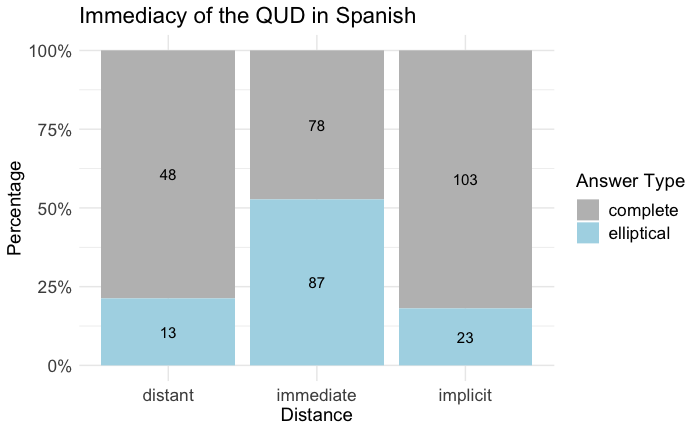
\includegraphics[width=0.8\textwidth]{Images/ES_immediacy.png}
    \caption{Immediacy of the QUD in Spanish}
    \label{fig:4:Plot1}
    % \label{fig:my_label}
\end{figure} 


To examine whether elliptical answers occurred significantly more often than complete answers within each QUD distance, binomial tests were conducted. In the immediate condition, the number of elliptical (87) and complete (78) answers did not differ significantly ($p > 0.05$). In contrast, in the distant condition, elliptical answers (13) were significantly less frequent than complete answers (48), $p < 0.001$. Similarly, in the implicit condition, elliptical answers (23) were significantly less frequent than complete answers (103), $p < 0.001$.

Thus, when the QUD is immediate, no significant difference can be observed in speakers' choice between a full and an elliptical answer (even though there is a slight preference for elliptical answers). This implies that in the case of an immediately-preceding question, Spanish speakers prefer to answer with strategies that contain an explicit BG (postverbal subject, an in situ subject, a cleft), or with strategies where only the focused subject is visible (reduced clefts or fragments). However, when the question is distant or implicit, a clear preference can be observed for answers with an overtly realized BG, suggesting that in those cases, speakers opt for strategies where they express more material. Thus, hypothesis (H1) is only partially confirmed for the Spanish data.

\section{Results for French} \label{sub:5.4}
As for the French results, participants produced 42\% (N=67) of the answers with an overt BG and 58\% (N=91) with an elided one in the \textsc{immediate} condition. In the \textsc{distant} condition, 77\% (N=100) are full items and 23\% (N=30) are elliptical ones. Lastly, the \textsc{implicit} condition is associated with 68\% (N=101) full answers and 32\% (N=47) elliptical strategies.

A Pearson's Chi-squared test showed that the proportion of elliptical versus complete answers differed significantly across QUD distance, $\chi^2(2, N = 436) = 53.8$, $p < 0.001$. Binomial tests within each distance condition revealed that, in the distant condition, elliptical answers (30) were significantly less frequent than complete answers (100), $p < 0.001$; in the immediate condition, elliptical answers (91) were significantly more frequent than complete answers (67), $p < 0.05$; and in the implicit condition, elliptical answers (47) were significantly less frequent than complete answers (101), $p < 0.001$. These results indicate that elliptical answers occur particularly often for immediate questions, while complete answers dominate for distant and implicit questions.

\begin{figure}

    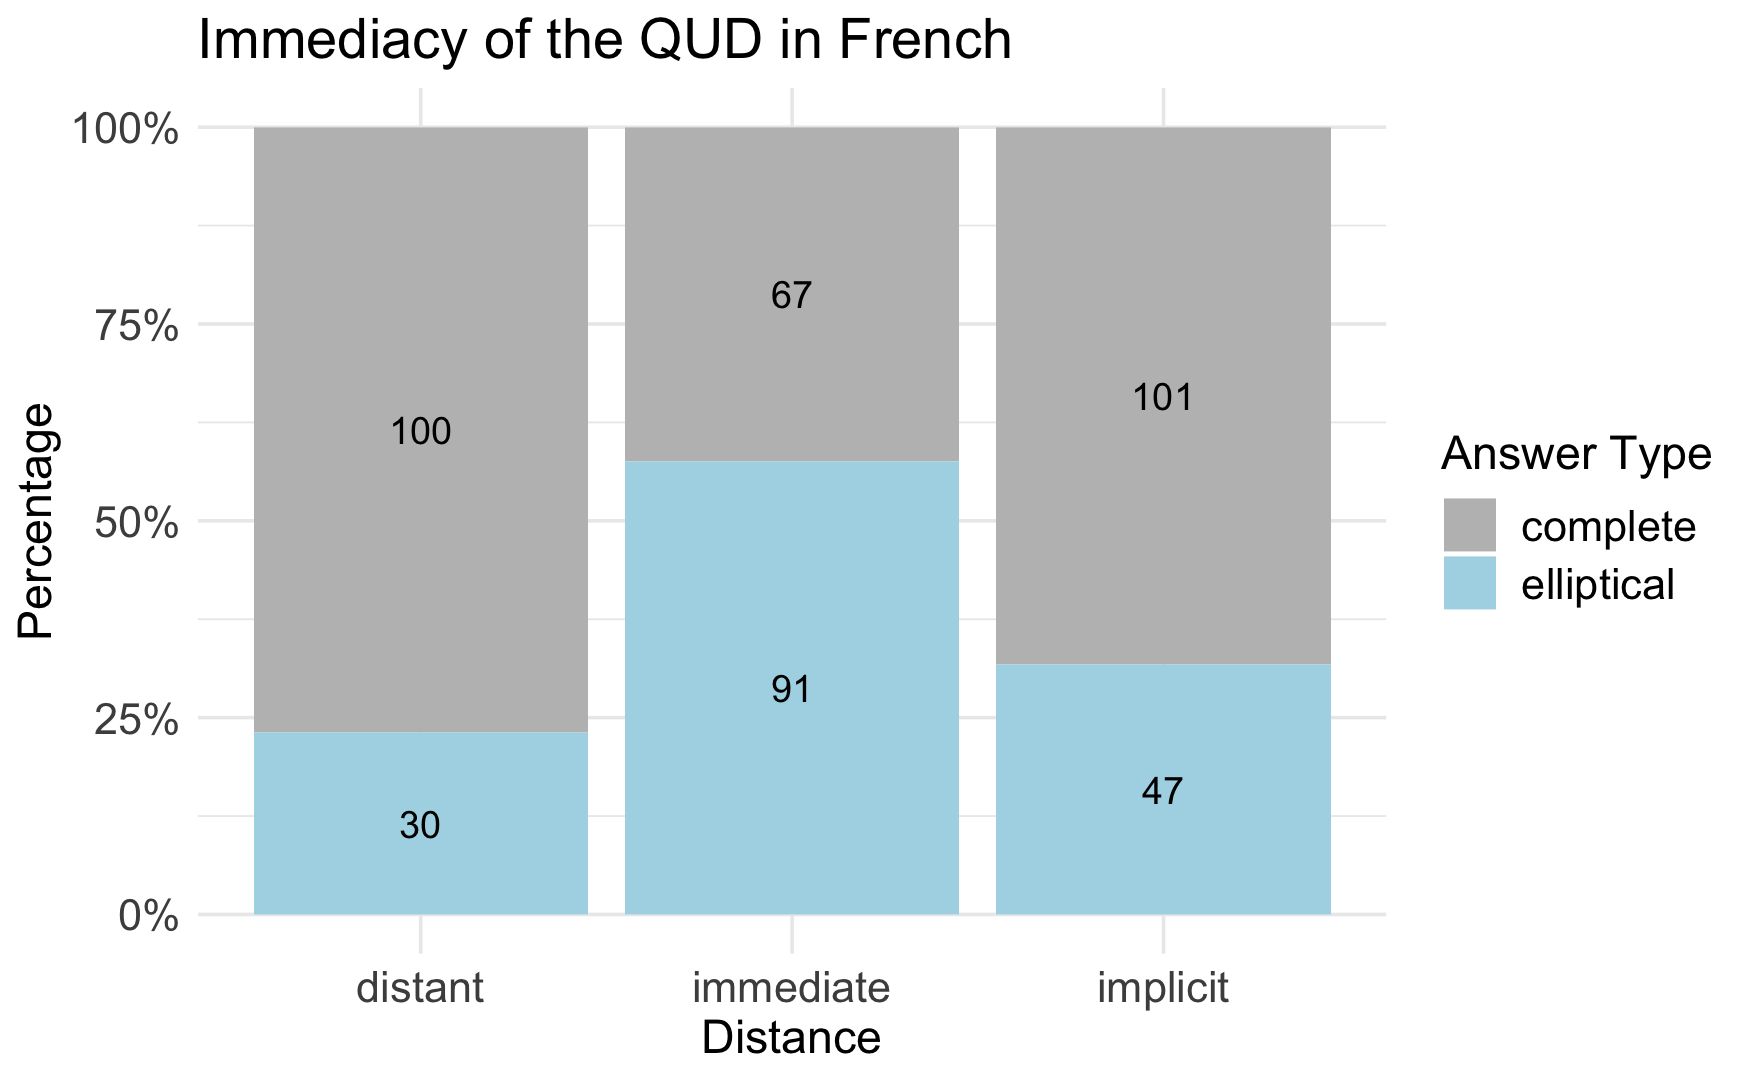
\includegraphics[width=0.8\textwidth]{Images/FR_immediacy.png}
    \caption{Immediacy of the QUD in French}
    \label{fig:4:Plot2}
    %\label{fig:my_label}
\end{figure} 

The results for the French sub-corpus reveal a different picture than the one visible for the Spanish data, at least in the \textsc{immediate} condition, where speakers show a significant preference for elliptical answers. Similarly to Spanish, in the cases of implicit or distant QUDs, there is a clear tendency to express more material, and to answer with a full strategy (as was the case in Spanish). The hypothesis (H1) is therefore fully confirmed for French.

\section{Comparative analysis} \label{sub:5.5}

Both the Spanish and the French dataset revealed interesting findings on the alternation between full and elliptical answers and their usage in spoken dialogues. The study showed that there is a clear effect of the degree of activation of the background proposition on the answer types produced by speakers. While elliptical answers are associated with a higher activation of the background material (even if to a lesser extent for the Spanish data), full answers are clearly more frequent when the BG proposition is less activated, like in the case of a distant or an implicit QUD.

This result is not surprising \textit{per se}, and several authors have already pointed out this correlation before, even if at a theoretical level (see section 5.1). However, to my recollection, these assumptions had never been operationalized or tested. In a dialogical setting, the QUD method gives clear insights into how the CG is managed, and how this constant evolution is reflected in speakers' linguistic choices. 

As mentioned in section 5.1, the idea of levels of activation of referents has already been acknowledged in many theories of CG content and CG management. Along the same lines as \textcite{ariel2001accessibility}, \textcite{chiarcos2011mental} in his ``iconicity principle in referential choice” claims that ``the  more  hearer  salient  a  discourse  referent  is,  the  less  marked  is  the  preferred referring expression” \parencite[201]{chiarcos2011mental}. Similar to \textcite{ariel2001accessibility}, this implies that there is an inverse relationship between the amount of linguistic coding and the assumed accessibility of the referent: the more accessible the  referent  is,  the  less  coding  is  needed. 

The corpus study conducted here shows that this inverse relationship is applicable not only to referents but also to other components of communication, such as propositions. Starting from the consideration that propositions can also be subject to different degrees of activation, this corpus study demonstrated how a higher level of salience of the proposition results in a smaller amount of linguistic material. Although this pattern is not as fine-grained as is the case for referring expressions, the results revealed that processes like deletion or overt realization of the proposition are actually indicators of different degrees of activation of the proposition itself. 
The background material is, by definition, a proposition that is already known and shared by speaker and hearer. However, the concept of givenness alone is not able to capture specific linguistic choices. For instance, empirical studies on referential choice  have shown that factors like distance from the last mention and competition (presence of intervening referents) might explain the phenomenon in a more comprehensive way (e.g., \cite{arnold2007effect}).
By applying the same principle to the BG proposition in dialogues, I demonstrated that factors such as distance from the QUD, intervening utterances or implicitness have a considerable impact on the choice of the answer produced.

\subsection{Why do French and Spanish differ?}
\label{sub:5.5.1}
The association between immediately preceding questions and elliptical answers, such as fragments or reduced clefts, is more pronounced in French (58\%) than in Spanish (49\%). This difference between the two languages may be due to differences in syntactic weight. As noted in \chapref{sec:3}, most full answers in French are cleft sentences, whereas in Spanish they are mainly postverbal subjects. From a syntactic perspective, there is a considerable difference between the two structures: a cleft sentence is a bi-clausal structure, where the BG material is encoded in the form of a relative clause. As such, clefts are ``heavy” and costly syntactic processes, and include additional lexical material (e.g., \textit{C'est... qui} `It is... that').
In the case of postverbal subjects, the background material consists of a predicate, and for transitive verbs, an object that can either be fully realized or cliticized. As postverbal subject constructions do not include additional lexical elements, they are inherently `lighter' than clefts. This difference could explain why, for Spanish immediate QUDs, there is no significant preference between full and elliptical answers. That is to say, repeating the entire background of a cleft construction, including the relative clause, requires more effort than repeating a verb and, for example, a complement.

A closer look at the Spanish data reveals that in many of the occurrences of immediate QUDs with full answers, the BG proposition, although repeated, is often reformulated. Consider (\ref{ex:4:13}):

\ea \label{ex:4:13}
\ea	\textit{¿Hay alguno} \uline{\textit{que no se lleve bien?}}\\
 ‘Is there anyone that doesn't get along with her?'
\ex \textit{Bueno a ver, había} {[\textit{las chicas del tercero}]\textsubscript{\textsc{foc.}}}\\
\normalsize \uline{\textit{que siempre tenían problemas con ella}}.\\
‘Well, let's see, there were the girls from the third floor that always had problems with her.' \hfill (\textit{sgs} Spanish, 21/118-119)   
\z \z

In (\ref{ex:4:13}), the BG proposition contained in the question \textit{llevarse bien} `to get along' is reformulated by speaker B, who prefers a different wording rather than the exact repetition (\textit{tener problemas} `to have problems'). This is evidence of the fact that, even in case of an answer with an expressed background, Spanish speakers tend to avoid the exact, same repetition of the BG proposition.

Moreover, as will be illustrated in \chapref{sec:5}, the majority of the verbs associated with postverbal subjects are monoargumental verbs, especially unaccusatives (as in (\ref{ex:4:14})). This implies that the BG proposition is often expressed only by a verb, and that repeating it -- although it has been immediately mentioned in the answer -- would not lead to the same infelicity in context as repeating an entire relative clause, as in the case of a cleft sentence.

\ea \label{ex:4:14}
\ea	\textit{¿Quién} \uline{\textit{ha fallecido}}?\\
 ‘Who died?'
\ex \uline{\textit{Ha fallecido}} {[\textit{la chica del segundo}]\textsubscript{\textsc{foc.}}}\normalsize\\
‘The girl from the second floor died.' \hfill (\textit{sgs} Spanish, 8/30-31)  
\z \z

Conversely, in French, the association between immediately preceding QUDs and elliptical answers is quite strong. However, while French speakers clearly prefer to omit the background material by opting for an elliptical strategy, full answers still appear in 42\% of cases with immediately preceding questions. As was the case in Spanish, in many instances, speakers tend to reformulate the background rather than repeat it exactly, as seen in example (\ref{ex:4:15}):

\ea \label{ex:4:15}
\ea \uline{\textit{Tu dis qu'il y a des gens qui sont venus hier?}}\footnote{Note that, in this case, the whole question contains background material. The presuppositional content would be `some people came here yesterday'. This being a yes-no question, the wh-question `who are these guys?' is implicit. However, the BG proposition still immediately precedes the critical item.}\\
 ‘You said that there are people that came here yesterday?'
\ex  \textit{Ouais, il y a} {[\textit{quatre gars}]\textsubscript{\textsc{foc}}} \uline{\textit{qui sont passés hier}}\normalsize.\\
‘Yes, there are four guys that stepped by yesterday.' 

\hfill (\textit{sgs} French, 83/231-232)    
\z \z


 Sometimes the repetition of the BG proposition is justified by the fact that the speaker adds a new element within the BG. This element could be an adverb, for instance, as (\ref{ex:4:16}):

\ea \label{ex:4:16}
\ea	\uline{\textit{Ils ont une femme de ménage qui vient les aider?}}\\
 `Do they have a housekeeper who comes and helps them?'
\ex \textit{Pendant une période }\textit{il y avait} {[\textit{une femme de ménage}]\textsubscript{\textsc{foc}}} \normalsize \uline{qui venait} \textit{\textbf{une fois par semaine}}.\\
`During a certain period there was a housekeeper who came once a week.' \hfill (\textit{sgs} French, 8/30-31)    
\z \z


\textcite{karssenberg2017oiseaux} had already noted this phenomenon in her data: ``However, it is important to note that in most specificational \textit{il y a}-clefts, the relative clause does not repeat a discourse-given variable verbatim: it usually contains at least a small piece of new information. In other words, the type of specificational cleft with a completely discourse-given relative clause, though often presented in analyses of clefts [...] is quite rare in my corpora. [...] In many cases, the extra piece of information is an evaluation on behalf of the speaker/writer [...].” \parencite[251]{karssenberg2017oiseaux}. 

It has to be pointed out that, according to the QUD approach, the new element corresponds to not-at-issue material since it does not answer the current QUD. Rather, it corresponds to an answer to an implicit sub-QUD. Nevertheless, this could be taken as another motivation for the speaker to repeat the full BG, instead of having only the focused element.

\tabref{tab:5.4} shows the differences between the two languages in terms of i) exact repetition of the BG (\ref{ex:4:14}), ii) reformulation (\ref{ex:4:15}) and iii) presence of a new element (\ref{ex:4:16}):

\begin{table}[ht]

\begin{tabular}{rrr}
  \lsptoprule
 & Spanish & French \\ 
  \midrule
Repetition & 56/78 (72\%) & 23/67 (34\%) \\ 
Reformulation & 13/78 (17\%)  & 24/67 (36\%) \\ 
New element & 9/78 (11\%)  &  20/67 (30\%)  \\ 
   \lspbottomrule
\end{tabular}
\caption{Comparative frequencies of different types of immediate QUDs}
\label{tab:5.4}
\end{table}

 As can be observed in the table, the cases of exact repetition of the BG proposition are more frequent in Spanish than in French. As mentioned above, this might be due to the fact that repeating an unaccusative verb is easier than repeating an entire relative clause. A closer examination of the French cases involving exact repetition shows that, among the 23 instances, many are contrastive, which explains the need to include additional material. Furthermore, an analysis of the cases in both languages that contain a new element indicates that these elements are typically adverbs or modifying clauses, which provide additional spatio-temporal information about the focused element.

\subsection{Focus and the economy principle of language} \label{sub:5.5.2}
Apart from these cases, it is safe to conclude that when the proposition is highly activated in the CG, its repetition is generally avoided because it would sound redundant and would lead to unnecessary prolixity. These results are in line with Levshina's \textit{Principle of Communicative Efficiency}, which states that speakers communicate in such a way as to ``minimize the cost-to-benefit ratio'' \parencite[30]{Levshina_2022}. In her theory, Levshina (\citeyear{Levshina_2022}) clarifies how successful communication leads to evoking cognitive effects, which in turn is necessary to influence others or adjust our own behaviour and which ultimately is what guarantees our survival as a group. The author also evokes the concept of accessibility, which, as previously mentioned, is an already established notion in the literature on referentiality \parencite{ariel2001accessibility, arnold2007effect}. In her model, this notion is extended to other contexts, referring to ``the ease with which some mental representations or forms can be activated in or retrieved from memory” \parencite[18]{Levshina_2022}. Levshina offers an overview of phenomena related to coding efficiency from various areas of grammar: referential expressions, grammatical markers, clause connectors and other complex syntactic phenomena, shortening of lexical material, as well as phonetic reduction/enhancement. 

When applying this principle to dialogical situations, it becomes evident that repeating the entire background proposition when it is highly activated may result in a loss of communicative efficiency, as it leads to redundancy and can sound unnatural. Instead, an elliptical answer is preferred, serving as an optimal strategy to maintain the flow of communication.
On the other hand, when the question is distant from the answer, the level of activation of the proposition decreases, especially when intervening utterances — such as sub-questions of the original QUD — are present. In such cases, speakers tend to provide more information to facilitate cooperation and ensure successful updating of the CG. By fully expressing the proposition and linking it to the focus constituent, speakers signal to the hearer that the focus must be interpreted in relation to a specific proposition, thereby minimizing ambiguity. 

Both the Spanish and the French data confirm this tendency, and reveal that, in the \textsc{distant} condition, the majority of the answers produced by both groups of speakers are complete strategies, i.e., answers with an expressed BG proposition.
A similar tendency can be observed in the case of implicit QUDs, even though, in this case, a different pragmatic process might be involved: accommodation. The pragmatic  notion  of  presuppositional  accommodation \parencite{lewis1979scorekeeping} is generally considered a communicational strategy through which the addressee adds the presupposed proposition to the set of all propositions which s/he assumes to be part of the interlocutors’ CG \parencite{beaver2007accommodation}. It is conceived as a universally-available adaptive mechanism to enhance communicative efficiency, and it is generally understood as a repair strategy: if a piece of information cannot be interpreted with respect to the current CG, then the current CG can minimally be changed in a way that it fits the requirement of the piece of information. The proposition is evoked, but not explicitly mentioned. However, speakers accommodate, the proposition is implicitly shared in the CG content, and the addressee reconstructs it in order to make his/her interlocutor's contribution informative.

The fact that both implicit and not immediate QUDs correlate with full answers is in line with the generalization that speakers express more when they presume that the hearer knows less, i.e., when they judge it useful  to clarify and to remind the addressee that the answer containing a particular referent has to be linked with a particular proposition.
Information structure is a continuous updating of  the  CG, and it is  dependent on the  speaker’s  intention  to communicate information based on what s/he assumed the hearer already knows. Therefore, in the case of implicit or distant questions, the cooperative speaker assumes that s/he has to express more material for a successful communication with the hearer. 

Conversely, in the case of an explicit and immediately-preceding QUD, there are enough contextual cues to determine what is going to follow, which implies that the hearer does not need to perform any costly operation. In this case, an elliptical answer type, like a fragment, is sufficient, whereas the need to use a more explicit focus-marking device such as a cleft diminishes. \textcite{zimmermann2011focus} also claim that, in the case of an explicit QUD, ``heavy” focus marking is less necessary and a more economical strategy is preferable.

The results issued in this chapter are also in line with a theory of economy of language \parencite{zipf1949human}, which emphasises the fundamental role played by the \textit{Principle of Least Effort}, which involves tending towards the minimum amount of effort necessary to achieve the maximum result.  Concerning linguistic behaviour, he distinguished the opposing pressures exerted by the speaker’s and the hearer’s economies of effort, the one oriented toward minimal linguistic articulation, the other toward maximal explicitness.
According to \textcite{carston2005note}, Zipf’s (\citeyear{zipf1949human}) speaker’s economy can be understood as a force pushing in the direction of a single word or sound that would express all possible meanings, thus sparing the speaker the mental effort that is involved in selecting the appropriate linguistic forms for the meanings s/he wants to convey.
The findings of this study confirm this tendency, showing that, in the presence of enough contextual cues for successful understanding, speakers prefer to express less. Conversely, they choose to express more when such cues are not as clear. 

Moreover, this study further emphasizes how our linguistic expressions are shaped by the types of questions they respond to. The QUD approach to focus is not new in itself. As discussed in \chapref{sec:2}, \textcite{roberts1996information} frames CG management as a discourse process driven by hierarchies of unresolved questions. While it is well-established that the use of ellipses is tied to attention and short-term memory, the systematic analysis linking ellipses (versus full forms) with the QUD framework presents an innovative contribution to this area of research.

\section{Summary} \label{sub:5.6}

In this chapter, I have investigated the alternation between full and elliptical answers in subject focus realization. I posited the hypothesis that the activation of the BG proposition is the factor determining such alternation, and I tested this hypothesis for both Spanish and French speakers. Although some differences can be found, both the Spanish and the French data show that elliptical answers are more frequent in contexts of high activation of the background material, whereas full strategies are preferred when such activation decreases.

As such, propositions are subject to the same iconicity principle \parencite{chiarcos2011mental} as referents, where an inverse relationship can be observed between the level of activation and the amount of linguistic coding.
To interpret the results, I have provided an account in terms of communicative efficiency. In particular, I claim that these communicative choices are subject to Levshina's principle of communicative efficiency \parencite{Levshina_2022} and to the Principle of Least Effort \parencite{zipf1949human}. Based on these findings, I propose that communicative strategies such as accommodation are reflected in speakers' linguistic choices, and in the way they decide to cooperate for a successful updating of the CG content.

Several authors have pointed out the fact that answers to questions in natural speech typically delete discourse-old information from  the question, or pronominalize arguments which cannot be grammatically deleted (e.g., \cite{krifka2008basic}). Examples can be found also in several unrelated languages, such as Northern Sotho \parencite{zerbian2007investigating} or Bantu languages \parencite{downing2016information}. Such tendencies, however, had never been tested for Spanish or French. By adopting the QUD method, I have suggested a possible means to operationalize claims that had been posited at a theoretical level. Thus, the ``immediacy” hypothesis is not necessarily exclusive to subject focus; rather, it can be extended to other types of constituent focus and, obviously, to other languages. Processes such as the activation of the background proposition or pragmatic accommodation are generally conceived of as universal, although their linguistic manifestation may vary across languages. This same hypothesis could be extended to object focus by exploring which structures emerge from a similar analysis and how they compare to the findings of this chapter. These questions, however, are outside the scope of this book, but remain nonetheless an interesting line of research for future work.

Although this chapter provides a pragmatic account for the alternation between full and elliptical strategies, it gives no indication as to why we find lan\-guage-internal and cross-linguistic syntactic variation to express the same function. In other words, why do Spanish postverbal subjects alternate with preverbal ones in the expression of subject focus? Why do we find different cleft types with the same IS-function? Are semantic and pragmatic factors responsible for the occurrence of one structure rather than the other? These questions are addressed in the next chapter, where I investigate the impact of different predictors on Spanish subject position and on French clefts from a language-internal and a cross-linguistic perspective.
